\documentclass[Rapport/Rapport_main.tex]{subfiles}
\begin{document}
\subsection{Scenarier}
Scenerierne beskriver systemets funktionalitet og adfærd, og tager udgangspunkt i User Story Distributionerne. Kun udvalgte distributioner vil blive gennemgået, de resterende henvises læseren til bilag \textbf{Arkitektur}. 
For at illustrere systemets adfærd bruges sekvensdiagrammer, som viser sammenspillet mellem aktør, applikation og database. 

\subsubsection{Oprettelse af bruger}
For at kunne anvende CarnGo applikationen, må brugeren oprette en profil. Brugerens information gemmes i databasen ved oprettelse. 
\begin{figure}[H]
    \centering
    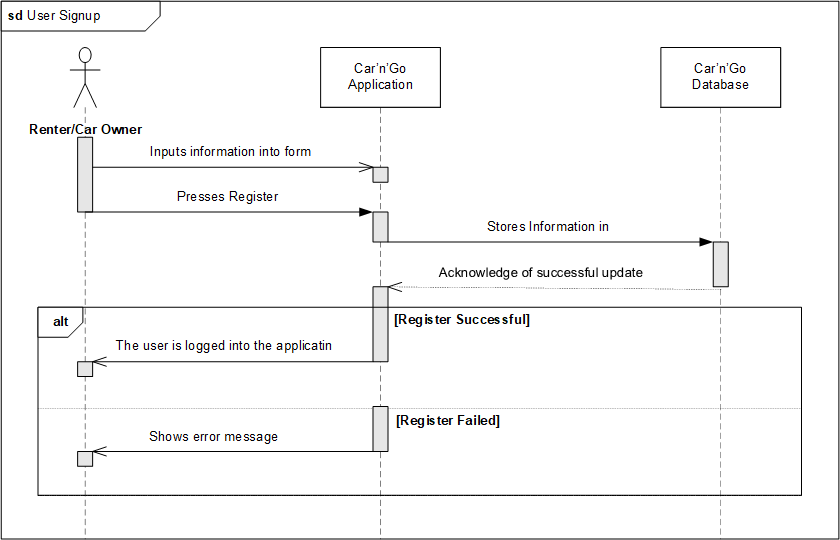
\includegraphics[width=\textwidth]{Arkitektur/Softwarearkitektur/User_Signup/graphics/UserSignupSD.png}
    \caption{Her ses et sekvens diagram for samspillet mellem lejer/udlejer, CarnGo applikationen samt databasen.}
    \label{fig:UserSignUpSD}
\end{figure}

\subsubsection{Oprettelse af bilprofil}
En bilprofil repræsenterer alt information omkring den bil som udlejes. En bruger med udlejerretigheder skal have mulighed for at oprette en bilprofil. En bruger med lejerretigheder kan ikke oprette bilprofiler. 
\begin{figure}[H]
    \centering
    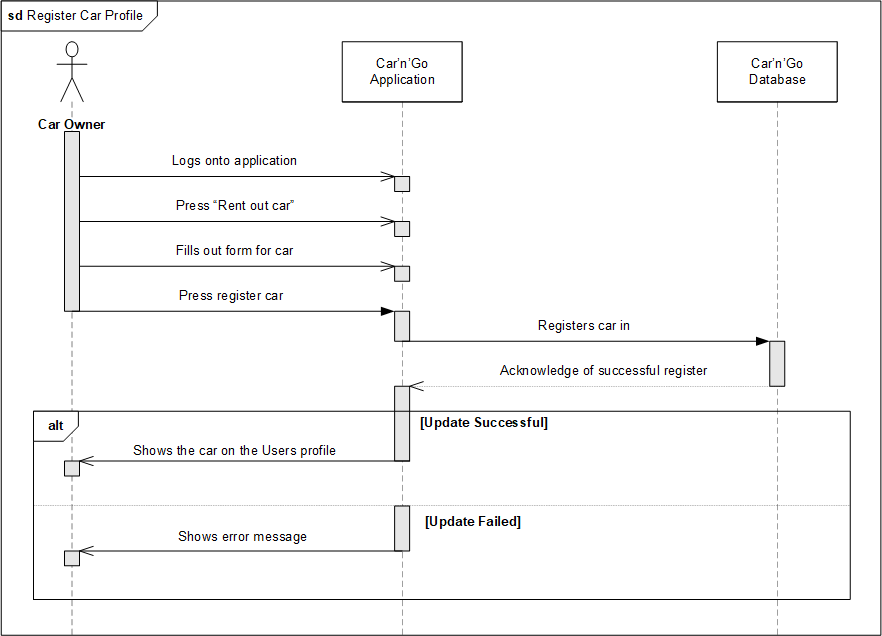
\includegraphics[width=1\textwidth]{Arkitektur/Softwarearkitektur/Car_registration/graphics/RegisterCarSD.png}
    \caption{Her ses et sekvensdiagram for samspillet mellem udlejer, applikation og database. }
    \label{fig:RegisterCarProfileSD}
\end{figure}


\subsubsection{Søgning}
Når en lejer ønsker at leje en bil, så skal han/hun søge efter en i applikationens katalog/database. I kataloget er lagret alle bilprofiler, som er sat til leje. 
\begin{figure}[H]
    \centering
    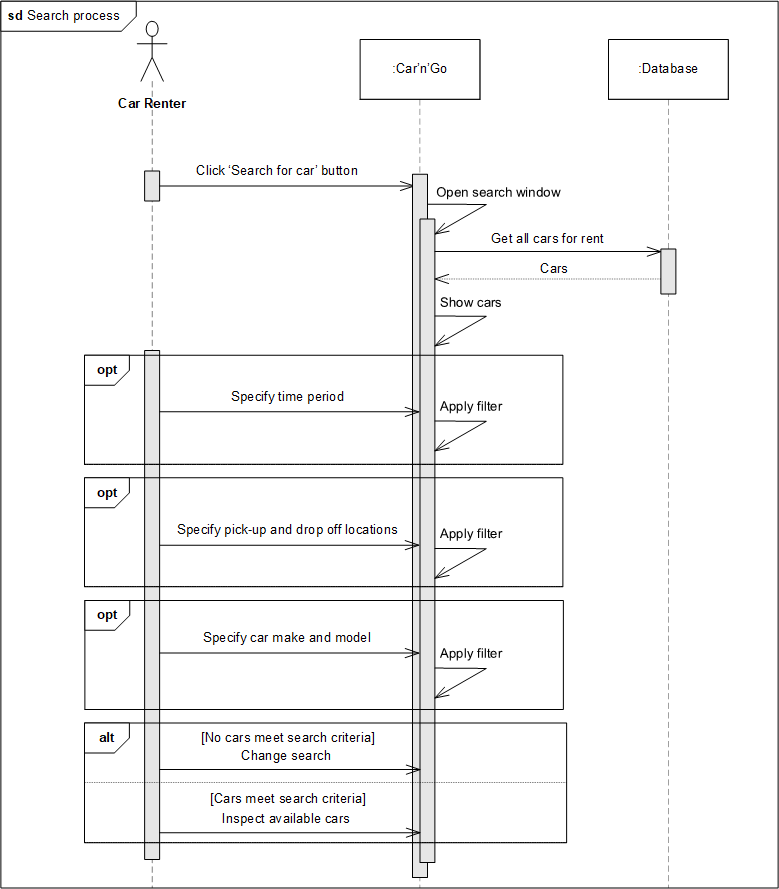
\includegraphics[width=1\textwidth]{Arkitektur/Softwarearkitektur/Searching/graphics/Search_Process_SD.png}
    \caption{Sekvensdiagram for søgning efter biler til leje. }
    \label{fig:SearchProcessSD}
\end{figure}

\subsubsection{Håndtering af udlejningsproces}
Efter at lejer har søgt i applikationens katalog, og har fundet en bil, som lejer ønsker at leje, så starter udlejningsprocessen. Dette realiseres med 3 trin: 
\begin{enumerate}
    \item Lejer anmoder udlejer om billeje 
    \item Udlejer godkender/forkaster anmodning om billeje 
    \item [Valgfri] Lejer tager kontakt til udlejer i forhold til udveksling af bil
\end{enumerate}
\begin{figure}[H]
    \centering
    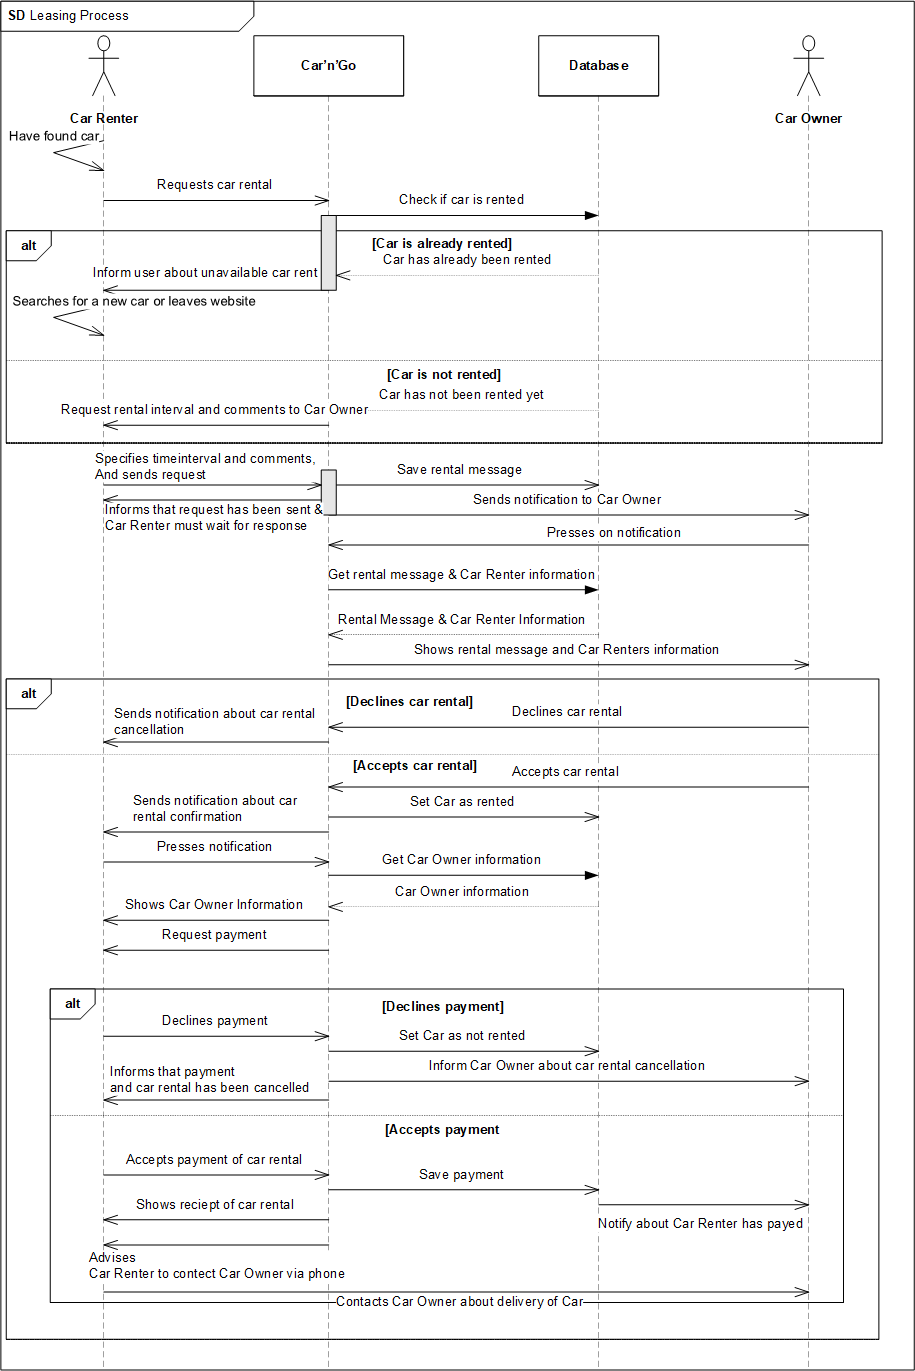
\includegraphics[width=1.1\textwidth]{Arkitektur/Softwarearkitektur/Leasing/graphics/Leasing_processSD.png}
    \caption{Sekvensdiagram for håndtering af udlejningsprocessen.}
    \label{fig:Leasing_processCD}
\end{figure}

\end{document}